\section{Постановка задачи}
Составить алгоритм и написать соответствующую ему программу, позволяющую:
\begin{itemize}
    \item выполнять операции сложения, вычитания и умножения в кольце вычетов;
    \item находить элементы, обратные к элементам, взаимно простым с модулем кольца;
    \item возводить в натуральную степень элементы кольца вычетов.
\end{itemize}


\clearpage
\section{Используемые инструменты}
Для решения вышеуказанной задачи были использованы следующие инструменты:
\begin{itemize}
    \item Основным ЯП был выбран Python версии 3.9.2;
    \item Для компиляции программы в бинарный файл .exe использован конвертер файлов Auto PY to EXE,
    который использует для своей работы PyInstaller.
\end{itemize}


\clearpage
\section{Общая структура библиотеки целых\\длинных чисел}
В библиотеке целых длинных содержится класс <<BigInt>>, в котором объявлены следующие методы:
\begin{itemize}
    \item Реализация алгоритма сложения в кольце вычетов.\\
    Алгоритм был реализован на основе работы сложения и нахождения остатка длинных чисел.
    Изменения касались лишь тех моментов, когда необходимо было реализовать логику кольца вычетов.
    \item Реализация алгоритма вычитания в кольце вычетов.\\
    Алгоритм был реализован на основе работы вычитания и нахождения остатка длинных чисел.
    Изменения касались лишь тех моментов, когда необходимо было реализовать логику кольца вычетов.
    \item Реализация алгоритма умножения в кольце вычетов.\\
    Алгоритм был реализован на основе работы умножения и нахождения остатка длинных чисел.
    Изменения касались лишь тех моментов, когда необходимо было реализовать логику кольца вычетов.
    \item Реализация алгоритма возведения в степень в кольце вычетов.\\
    Алгоритм был реализован на основе работы бинарном алгоритме возведения в степень и нахождения остатка длинных чисел.
    Изменения касались лишь тех моментов, когда необходимо было реализовать логику кольца вычетов.
    \item Реализация расширенного алгоритма Евклида для поиска НОД двух длинных целых чисел, а также коэффициентов.\\
    Данный алгоритм был реализован для его дальнейшего использования в алгоритме нахождения обратного элемента в кольце вычетов.
    Этот алгоритм, в отличие от других реализаций алгоритмов поиска НОД, является методом класса, а не функцией.
    \item Реализация нахождения обратного элемента в кольце вычетов.\\
    Алгоритм был реализован на основе работы сложения, вычитания и расширенного алгоритма Евклида для поиска НОД длинных чисел.
    В случае использования расширенного алгоритма Евклида для поиска НОД от данного метода требуются коэффициенты.
\end{itemize}

Класс <<BigInt>> содержит в себе два основных поля:
\begin{enumerate}
    \item Поле хранения числа <<value>>.\\
    Представляет собой переменную типа строка, в котором содержится число экземпляра класса;
    \item Поле хранения знака числа <<is\_neg>>.\\
    Представляет собой переменную типа bool, в которой содержится информация о знаке числа.
    Значение True эквивалентно отрицательному числу, значение False - положительному;
\end{enumerate}

Создания экземпляра класса <<BigInt>> происходит следующие способами:
\begin{itemize}
    \item Создание экземпляра класса без передачи аргументов. Числовое значение такого экземпляра будет равно нулю.
    \begin{lstlisting}
a = BigInt()\end{lstlisting}
    \item Создание экземпляра класса с передачей в аргумент строки, которая может валидно быть приведена к типу целого числа.
    \begin{lstlisting}
a = BigInt('-1234567890')  # a = -1234567890
b = BigInt('1234567890')   # b = 1234567890
d = BigInt('0')            # d = 0\end{lstlisting}
    \item Создание экземпляра класса с передачей в аргумент целого числа.
    \begin{lstlisting}
a = BigInt(-1234567890)  # a = -1234567890
b = BigInt(1234567890)   # b = 1234567890
d = BigInt(0)            # d = 0\end{lstlisting}
    \item Создание экземпляра класса с передачей в аргумент экземпляра класса <<BigInt>>.
    \begin{lstlisting}
a = BigInt(-1234567890)  # a = -1234567890
b = BigInt(a)            # b = -1234567890\end{lstlisting}
\end{itemize}


\clearpage
\section{Примеры работы библиотеки}
В качестве примера работы будут использоваться прямые вызовы методов класса <<BigInt>>.

Пусть даны:
\begin{itemize}
    \item два длинных числа $x1$ и $y1$, сохраненных в экземпляр класса <<BigInt>>;
    \item два обычных длинных числа $x2$ и $y2$, для степенных операций;
    \item длинное число N, которое будет использовано в качестве модуля.
\end{itemize}

    \begin{lstlisting}
x1 = BigInt('99999999999999999999')
y1 = BigInt('11111111111111111111')
x2 = BigInt('99')
y2 = BigInt('11')
N = BigInt('12345678998765432')\end{lstlisting}

    \begin{itemize}
        \item Выполняем сложение в кольце вычетов:
        \begin{lstlisting}
print(BigInt.ring_add(x1, y1))\end{lstlisting}
        Вывод: $122222223110$
        \item Выполняем вычитание в кольце вычетов:
        \begin{lstlisting}
print(BigInt.ring_sub(x1, y1))\end{lstlisting}
        Вывод: $97777778488$
        \item Выполняем умножение в кольце вычетов:
        \begin{lstlisting}
print(BigInt.ring_mul(x1, y1))\end{lstlisting}
        Вывод: $21010000081689$
        \item Выполняем нахождения обратного элемента в кольце вычетов:
        \begin{lstlisting}
print(BigInt.ring_inv_el(x1, N))\end{lstlisting}
        Вывод: $5264157999473642$
        \item Выполняем возведение в степень в кольце вычетов:
        \begin{lstlisting}
print(BigInt.ring_pow(x2, y2))\end{lstlisting}
        Вывод: $12182065501559763$
    \end{itemize}

\clearpage
\section{Вывод}
Мною был составлен алгоритм (в виде блок-схемы) и написана на языке Python программа, позволяющая:
\begin{itemize}
    \item производить сложение в кольце вычетов двух длинных чисел;
    \item производить вычитания в кольце вычетов двух длинных чисел;
    \item производить умножения в кольце вычетов двух длинных чисел;
    \item производить возведение в степень числа в кольце вычетов;
    \item находить НОД двух длинных чисел, а также коэффициенты;
    \item находить обратный элемент в кольце вычетов;
\end{itemize}

\clearpage
\section{Блок-схема методов библиотеки}
Ниже представлены блок-схемы методов в следующем порядке:
\begin{enumerate}
    \item Метод нахождения суммы в кольце вычетов двух длинных чисел;
    \item Метод нахождения разности в кольце вычетов двух длинных чисел;
    \item Метод нахождения произведения в кольце вычетов двух длинных чисел;
    \item Метод, позволяющий возводить в степень числа в кольце вычетов;
    \item Метод нахождения НОД двух длинных чисел, а также коэффициенты;
    \item Метод нахождения обратного элемента в кольце вычетов.
\end{enumerate}
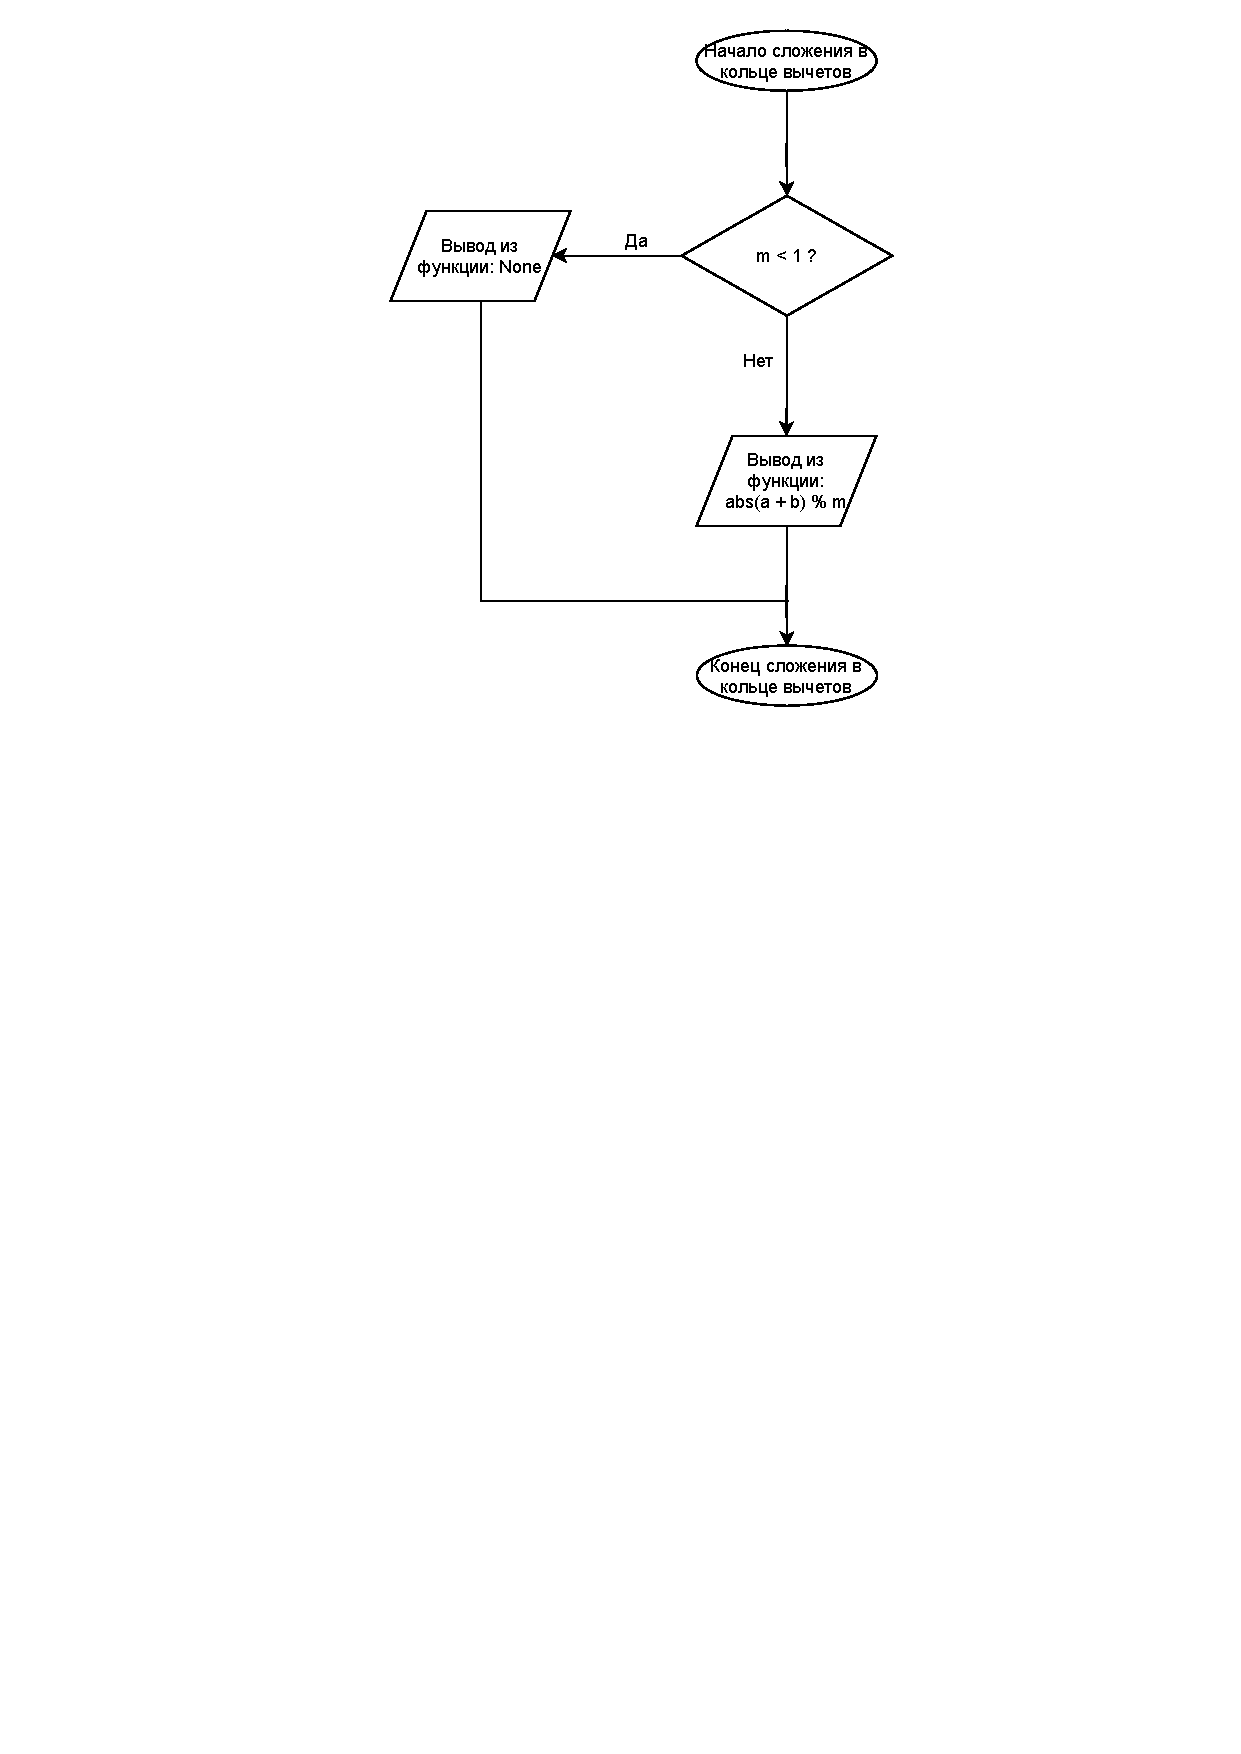
\includepdf[pages=-]{./Flowchart.pdf}
